\documentclass{article}
\usepackage[UTF8]{ctex}  % 使用中文支持包
\usepackage[a4paper, margin=1in]{geometry}  % 设置纸张大小和边距
\usepackage{anyfontsize}  % 解决字体大小报错问题
\usepackage{fancyhdr}  % 设置页眉、页脚、页码
\usepackage{longtable}  % 支持长表格

\usepackage{amsmath}  % 数学公式支持
\usepackage{cases}  % 支持联立编号

\usepackage{graphicx}  % 插入图片支持
\usepackage{float}  % 设置图片浮动位置
\usepackage{subfigure}  % 插入多图时用子图显示

\usepackage{listings}  % 代码块支持
\usepackage{xcolor}  % 设置代码块颜色

\usepackage[hyphens]{url}  % 支持链接换行
\usepackage{hyperref}  % 超链接支持
\usepackage{lastpage}  % 添加lastpage包
\usepackage{gbt7714}  %国标参考文献
\bibliographystyle{gbt7714-numerical}
\hypersetup{
    hidelinks,
    colorlinks=true,
    allcolors=black,
    pdfstartview=Fit,
    breaklinks=true
}

\title{射线源导论-第八周作业}
\author{\LaTeX\ by\ Jerry\ }
\date{\today}
\pagenumbering{arabic}

\begin{document}
\pagestyle{fancy}

\fancyhead[L]{Jerry}
\fancyhead[C]{射线源导论-第八周作业}
\fancyhead[R]{\today}
\fancyfoot[C]{Page \thepage/\pageref{LastPage}}

\section*{第八周课程作业}

\subsection*{\emph{Mo(钼)和W(钨)是常用的X光管阳极材料,请通过查找资料计算:}}

\begin{enumerate}
    \item \emph{Mo和W的k$\alpha$射线能量,以及激发该特征射线所需最低电子能量}
    \item \emph{尝试给出X-ray tube高压为50keV、100keV、150keV时能谱示意图}
    \item \emph{考虑到产生的X-ray光子约40\%的被靶自吸收,最终电子能量转为X射线能量的效率约为多少?}
\end{enumerate}

(1)

$$E_{k\alpha_1}(\text{Mo}) = 17.478 , \text{keV},\ \ \ E_{k\alpha_2}(\text{Mo}) = 17.373 , \text{keV}$$
$$E_{k\alpha_1}(\text{W}) = 59.310 , \text{keV},\ \ \ E_{k\alpha_2}(\text{W}) = 57.973 , \text{keV}$$
$$E_K(\text{Mo}) = 20.002 , \text{keV},\ \ \ E_K(\text{W}) = 69.503 , \text{keV}$$

(2)

\begin{figure}[htbp]
    \centering
    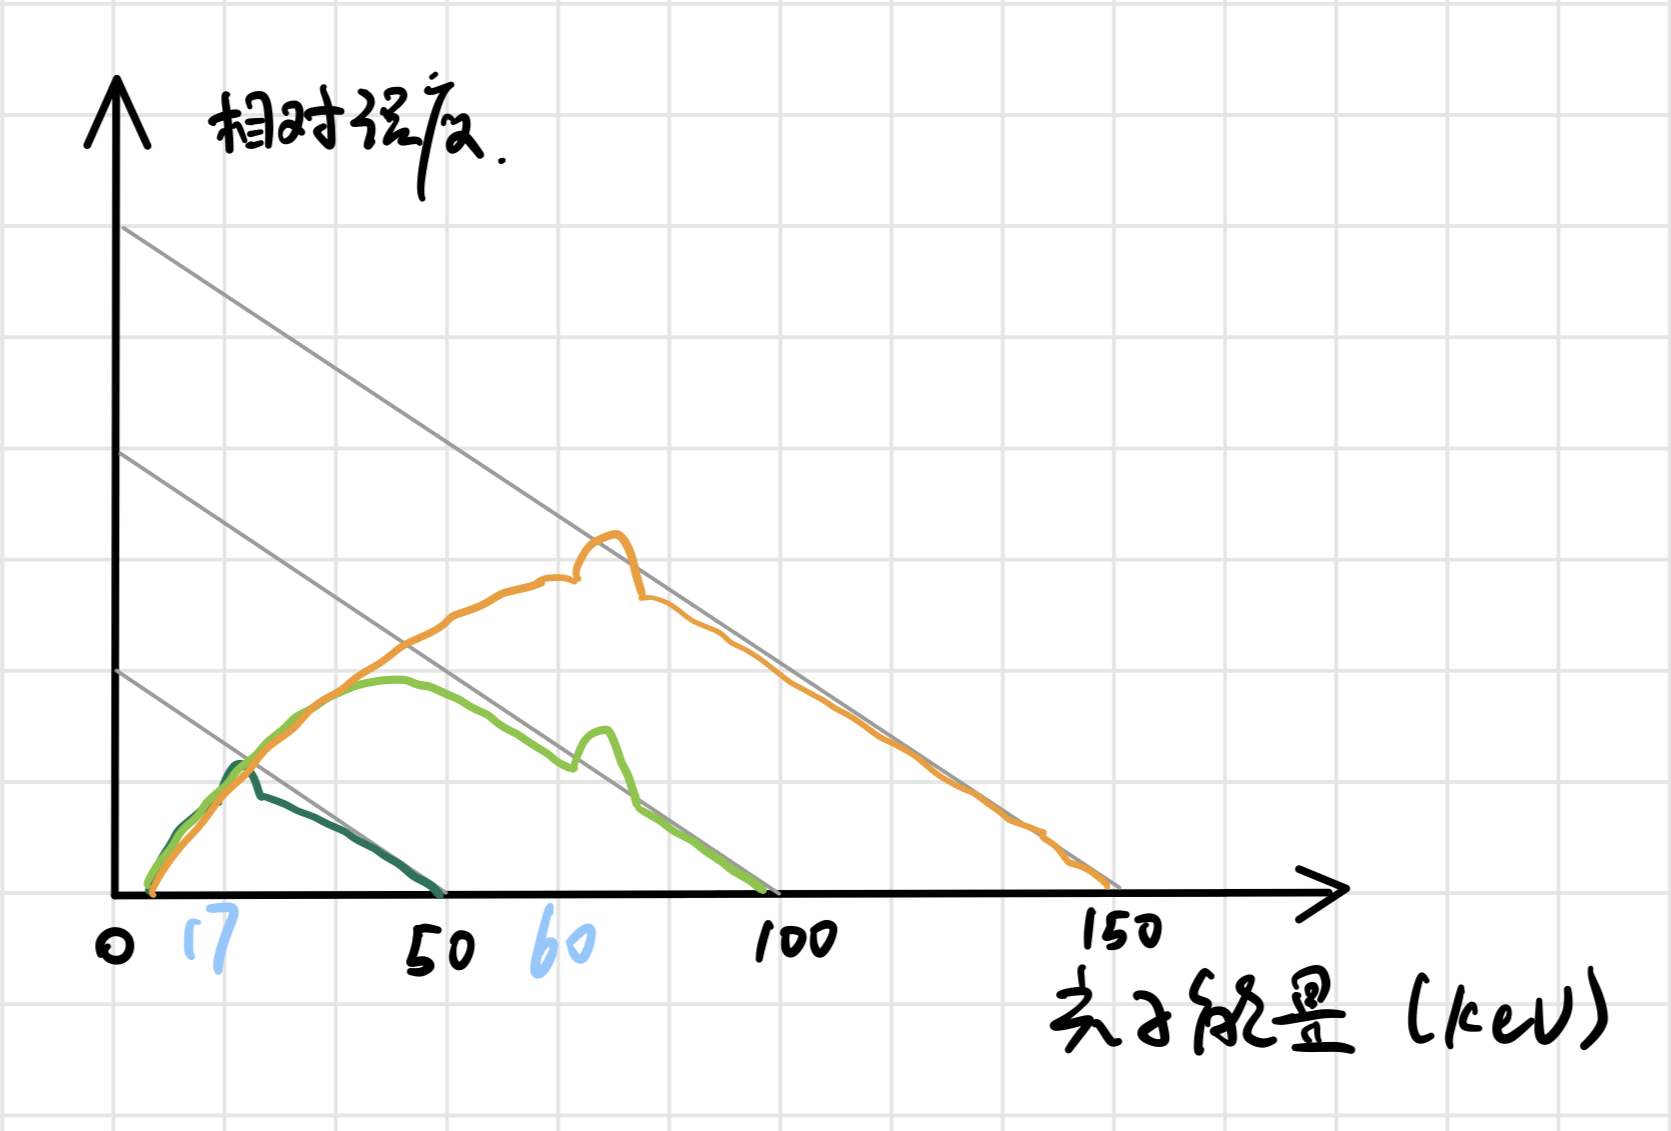
\includegraphics[width=0.5\textwidth]{./img/2.jpg}
    \caption{X-ray tube高压为50keV、100keV、150keV时能谱示意图}
    \label{fig:2}
\end{figure}

(3)

由于$\eta=C_{n}ZV=1.1\cdot10^{9}\cdot Z\cdot V$,代入$Z(Mo)=42,Z(W)=72$,可得:

50keV

$$\eta(Mo)=1.1\cdot10^{-9}\cdot50\cdot10^{3}\cdot42\cdot40\%=0.0924\%$$
$$\eta(W)=1.1\cdot10^{-9}\cdot50\cdot10^{3}\cdot74\cdot40\%=0.1628\%$$

100keV

$$\eta(Mo)=1.1\cdot10^{-9}\cdot100\cdot10^{3}\cdot42\cdot40\%=0.1848\%$$
$$\eta(W)=1.1\cdot10^{-9}\cdot100\cdot10^{3}\cdot74\cdot40\%=0.3256\%$$

150keV

$$\eta(Mo)=1.1\cdot10^{-9}\cdot150\cdot10^{3}\cdot42\cdot40\%=0.2772\%$$
$$\eta(W)=1.1\cdot10^{-9}\cdot150\cdot10^{3}\cdot74\cdot40\%=0.4884\%$$

\end{document}
